%& -shell-escape
\documentclass[a4paper, 12pt]{article}
\usepackage{barinovlab}
\setlength\itemsep{0pt}
\begin{document}
\thispagestyle{empty}
\begin{center}
    \textit{Федеральное государственное автономное образовательное\\ учреждение высшего образования }

    \vspace{0.5ex}

        \textbf{«Московский физико-технический институт\\ (национальный исследовательский университет)»}
\end{center}

\vspace{10ex}

\begin{center}
    \vspace{13ex}

    \so{\textbf{Лабораторная работа №-.-.-}}

    \vspace{1ex}

    по курсу общей физики

    на тему:

    \textbf{\textit{<<>>}}

    \vspace{30ex}

    \begin{flushright}
        \noindent
        \textit{Работу выполнил:}\\  
        \textit{Баринов Леонид \\(группа Б02-827)}
    \end{flushright}
    \vfill
    Долгопрудный \\2019
\newpage
\setcounter{page}{1}
\fancyhead[R]{\nouppercase{\leftmark}}	
\end{center}

\section{Аннотация}
В работе будут исследованы методы получения анализа поляризованного
света.

\section{Теоретические сведения}
\subsection*{Получение эллиптически поляризованного света}
Эллиптически поляризованной свет можно получить из линейно
поляризованного с помощью двоякопреломляющих кристаллических
пластинок.

\begin{wrapfigure}{r}{0.3\linewidth}
    \includegraphics[width=\linewidth]{1}
    \caption{Разложение линейно поляризованного света по главным
    направлениям двоякопреломляющей пластинки}
    \label{fig:1}
\end{wrapfigure}

Двоякопреломляющая пластинка имеет два взаимно перпендикулярных
главных направления, совпадающих с осями эллипсоида диэлектрической
проницаемости. Волны, поляризованные вдоль главных направлений,
распространяются в пластинке с разными скоростями, не изменяя
характера своей поляризации. Эти волны называются главными. Мы будем
обозначать показатели преломления для главных волн через $n_x$ и
$n_y$, где $x$ и $y$ --- главные направления кристаллической пластинки
\fig{fig:1}.

Пусть на пластинку падает линейно поляризованная волна, электрический
вектор которой ориентирован под некоторым углом $\alpha$ к оси $x$.
Разложим вектор $\vv{E}$ на составляющие $E_x$ и $E_y$. На входе
пластинки $E_x$ и $E_y$ находятся в фазе. На выходе из-за разности
скоростей между ними появляется разность хода $d(n_x-n_y)$, при этом
сдвиг фаз определяется соотношением:
\begin{equation}
    \Delta \phi = \frac{2\pi}{m}= kd(n_x-n_y)
    \label{eq:1}
\end{equation}
где $k$ --- волновое число (в пустоте), $d$ --- толщина
кристаллической пластинки.

Рассмотрим практически важные частные случаи

\begin{wrapfigure}[13]{l}{0.3\linewidth}
    \includegraphics[width=\linewidth]{2}
    \caption{Поворот направления колебаний с помощью пластинки в
    $\lambda/2$}
    \label{fig:2}
\end{wrapfigure}

Пластинка дает сдвиг фаз $2\pi$ (пластинка в длину волны $\lambda$). В
результате сложения волн на выходе пластинки образуется линейно
поляризованная волна с тем же направлением колебаний, что и в падающей
волне.

Пластинка дает сдвиг фаз $\pi$ (пластинка в полдлины волны
$\lambda/2$). На выходе пластинки снова образуется линейно
поляризованная волна. Направление $bb'$ колебаний этой волны повернуто
относительно направления $aa'$ колебаний падающей волны (\fig{fig:2}).
Направление $bb'$ является зеркальным отображением направления $aa'$
относительно одного из главных направлений пластинки. Такую пластинку
используют для поворота направления колебаний линейно поляризованного
света.

Пластинка создает между колебаниями сдвиг фаз $\pi/2$ (пластинка в
четверть длины волны). При сложении двух взаимно перпендикулярных
колебаний, имеющих разность фаз $\pi/2$, образуется эллипс, главные
оси которого совпадают с координатными осями $x$ и $y$. При равенстве
амплитуд $E_x^\text{max} = E_y^\text{max}$ возникает круговая
поляризация.

\subsection*{Пластинка чувствительного оттенка}

\begin{wrapfigure}{l}{0.25\linewidth}
    \includegraphics[width=\linewidth]{3}
    \caption{Пластинка чувствительного оттенка}
    \label{fig:3}
\end{wrapfigure}

Пластинка имеет форму стрелы (\fig{fig:3}), вдоль оси которой
расположено главное направление, соответствующее большей скорости
распространения.

Если между скрещенными поляроидами поместить пластинку чувствительного
оттенка ($\lambda$) и пластинку $\lambda/4$ так, чтобы их главные
направления совпадали, цвет пластинки изменится. Если у пластинки
чувствительного оттенка и пластинки в $\lambda/4$ совпадут главные
направления, соответствующие большей скорости распространения, то
разность хода между $E_x$ и $E_y$ для зеленого света составит уже
$5\lambda/4$. Это соответствует разности хода в $\lambda$ для света с
большей длиной волны. При освещении этих пластинок белым светом теперь
погасится не зеленая, а красная часть спектра, и проходящий свет будет
казаться зеленовато-голубым. Если же главные направления,
соответствующие большей скорости распространения, у пластинки
чувствительного оттенка и у пластинки в $\lambda/4$ окажутся
перпендикулярными, то проходящий свет приобретет оранжево-желтую
окраску.

\subsection*{Интерференция поляризованных лучей}
\begin{wrapfigure}{r}{0.3\linewidth}
    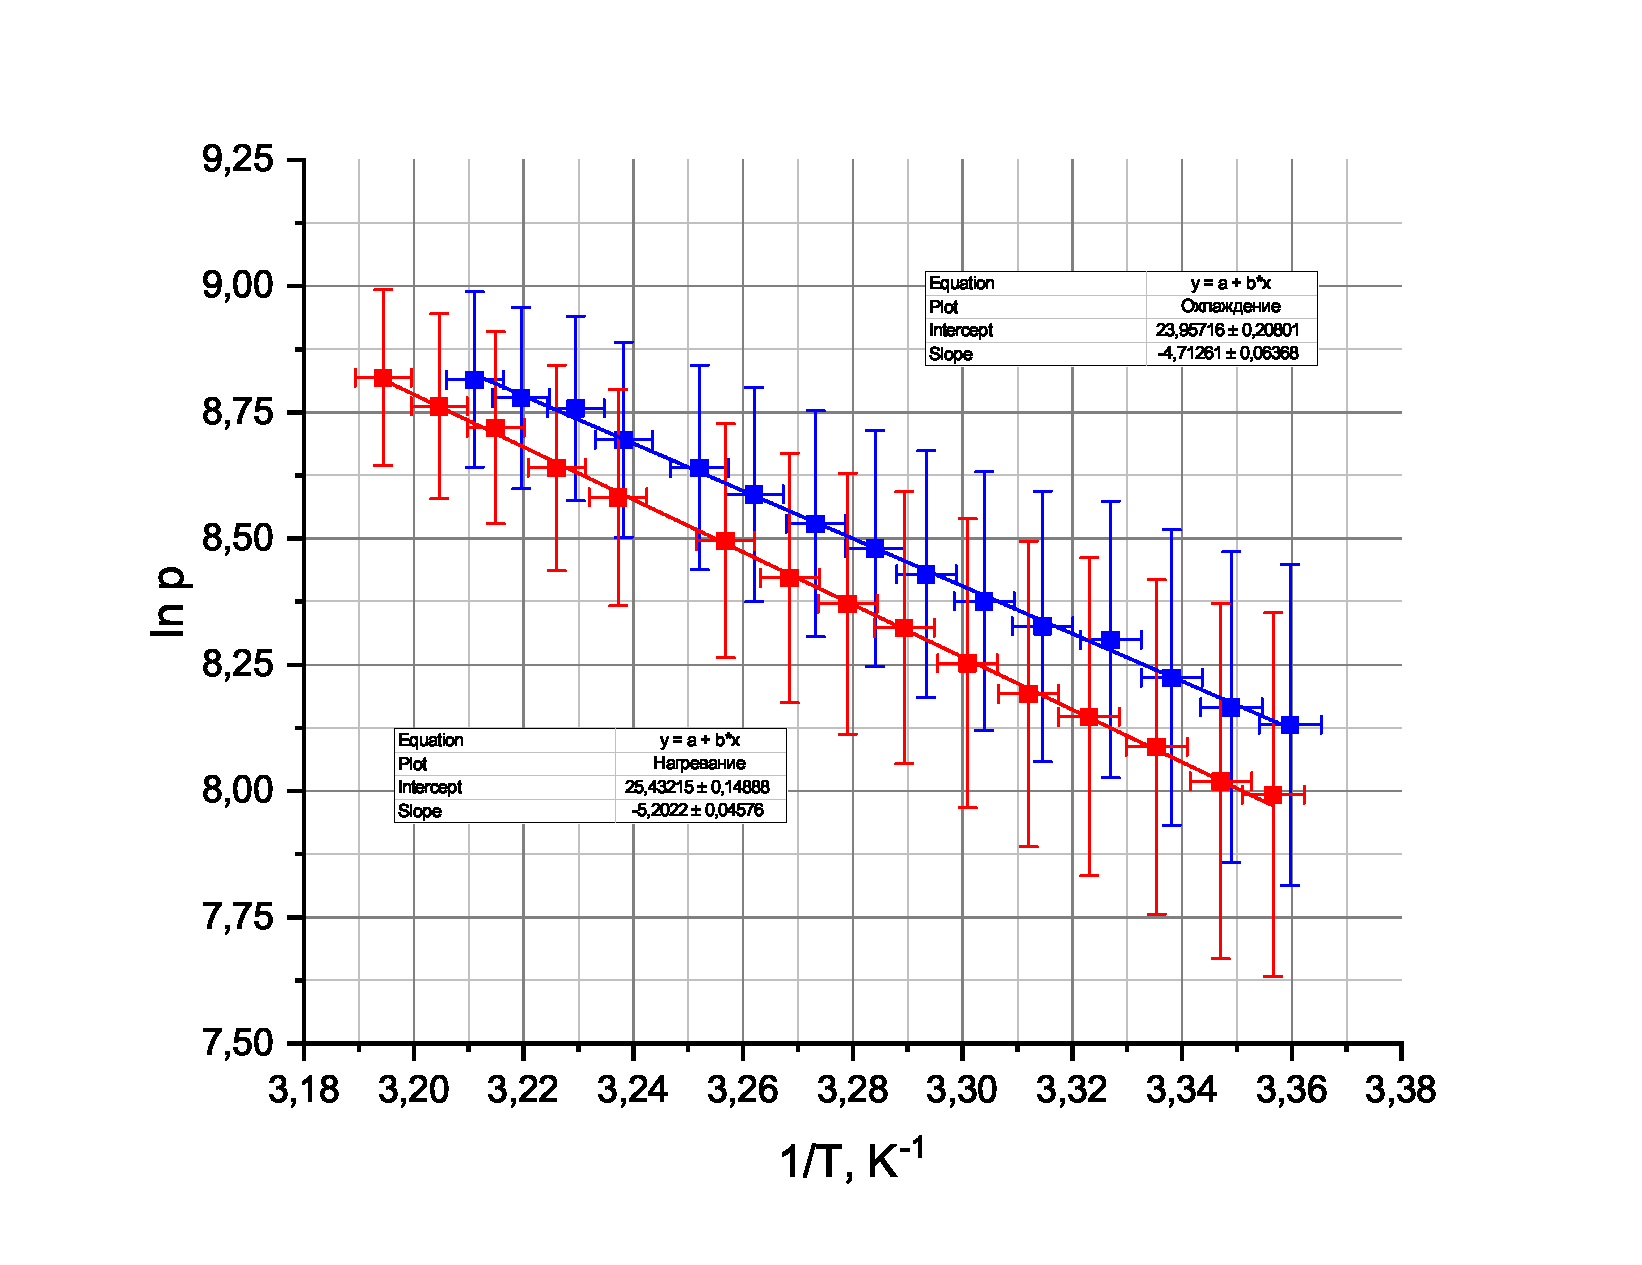
\includegraphics[width=\linewidth]{4}
    \caption{К объяснению интерференции поляризованных лучей}
    \label{fig:4}
\end{wrapfigure}

На \fig{fig:4} представлена схема для случая скрещенных поляроидов.

Здесь $p_1p_1'$ --- разрешенное направление колебаний поляризатора
(первого поляроида); $x, y$ --- координатная система, связанная с
главными направлениями двоякопреломляющей пластинки; $p_2p_2'$ ---
разрешенное направление колебаний анализатора (второго поляроида).
Волны $E_x$ и $E_y$ на выходе из пластинки когерентны, но не могут
интерферировать, так как $\vv{E}_x \perp \vv{E}_y$. Волны $E_1$ и
$E_2$ на выходе второго поляроида также являются когерентными и к тому
же поляризованы в одной плоскости. Эти волны интерферируют между
собой. Результат интерференции определяется зависящим от длины волны
сдвигом фаз между $E_1$ и $E_2$. В результате интерференции
поляризованных лучей пластинка, освещаемая белым светом, кажется
окрашенной.

Если поворачивать двоякопреломляющую пластинку, расположенную между
скрещенными поляроидами, то соотношение амплитуд волн $E_1$ и $E_2$ и
разность фаз между ними не изменяются. Это означает, что цвет
пластинки при ее поворотах не меняется, а меняется только
интенсивность света. За один оборот пластинки интенсивность четыре раза
обращается в нуль --- это происходит при совпадении главных направлений
$x$ и $y$ с разрешенными направлениями колебаний поляроидов.

Ели же двоякопреломляющую пластинку оставить неподвижной, а второй
поляроид повернуть так, чтобы разрешенные направления $p_1p_1'$ и
$p_2p_2'$ совпали, то волны $E_1$ и $E_2$ приобретают дополнительный
фазовый сдвиг на $\pi$ для всех спектральных компонент; при этом их
амплитуды изменятся так, что цвет пластинки изменится на
дополнительный.

\section{Оборудование}
\textbf{В работе используются:} оптическая скамья с осветителем,
зеленый светофильтр; два поляроида; черное зеркало; полированная
эбонитовая пластинка; стопа стеклянный пластинок; слюдяные пластинки
разной толщины; пластинки 1/4 и 1/2 длины волны; пластинка в одну
длину волны для зеленого света (пластинка чувствительного оттенка).






\section{Результаты измерений и обработка результатов}
\subsection*{Показатель преломления эбонита}

\begin{wrapfigure}{r}{0.4\linewidth}
    \includegraphics[width=\linewidth]{5}
    \caption{Определение разрешенного направления поляроида}
    \label{fig:5}
\end{wrapfigure}

Определим разрешенные направления поляроидов. Для этого разместим на
оптической скамье осветитель $S$, поляроид $P_1$ и черное зеркало
(\fig{fig:5}). Поворачивая поляроид вокруг направления луча, а черное
зеркало вокруг вертикальной оси, методом последовательных приближений
добьемся наименьшей яркости отраженного пятна. 

Определим показатель преломления эбонита. Для этого поставим на скамью
вместо черного зеркала эбонитовую пластину и определим по лимбу угол
Брюстера для эбонита:
\[
    \theta = (53\pm 2)^\circ 
\]
Рассчитаем показатель преломления по формуле $n = \tg \theta$:
\[
    n = 1,33\pm 0,10
\]
Табличное значение показателя преломления эбонита:
\[
    n^\text{т} = 1,6 - 1,7
\]

\newpage
\subsection*{Характер поляризации света в преломленном и отраженном от
стопы лучах}

\begin{wrapfigure}[9]{l}{0.4\linewidth}
    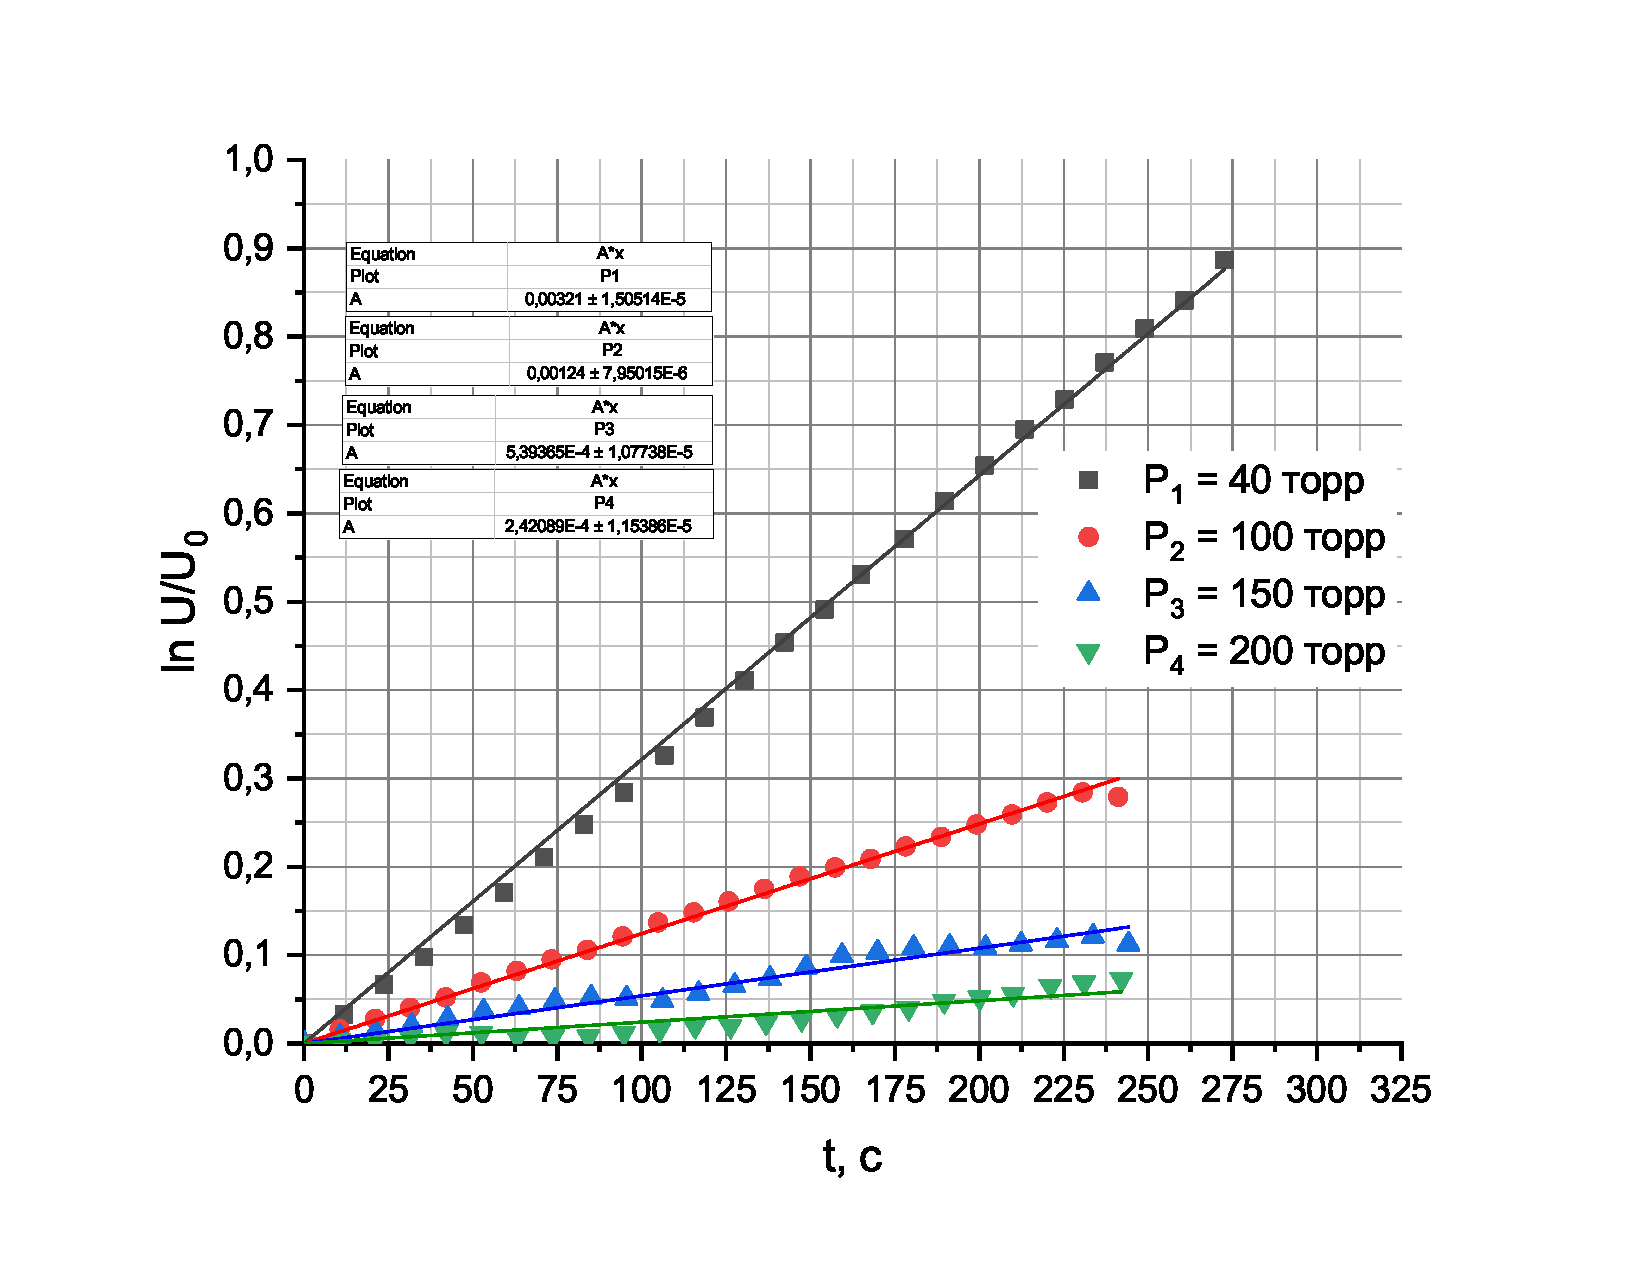
\includegraphics[width=\linewidth]{6}
    \caption{Исследование стопы}
    \label{fig:6}
\end{wrapfigure}

Поставим вместо эбонитового зеркала \ffig{fig:5} стопу стеклянных
пластинок под углом Брюстера.

Осветим стопу неполяризованным светом и, рассматривая через поляроиды
\ffig{fig:6} отраженный от стопы и преломленные лучи, определим в них
ориентацию $\vv{E}$

Получаем, что он отклоняется от направления распространения света на
угол $\pi/2$.

\subsection*{Двоякопреломляющие пластины}

\begin{wrapfigure}[7]{r}{0.35\linewidth}
    \vspace{-20pt}
    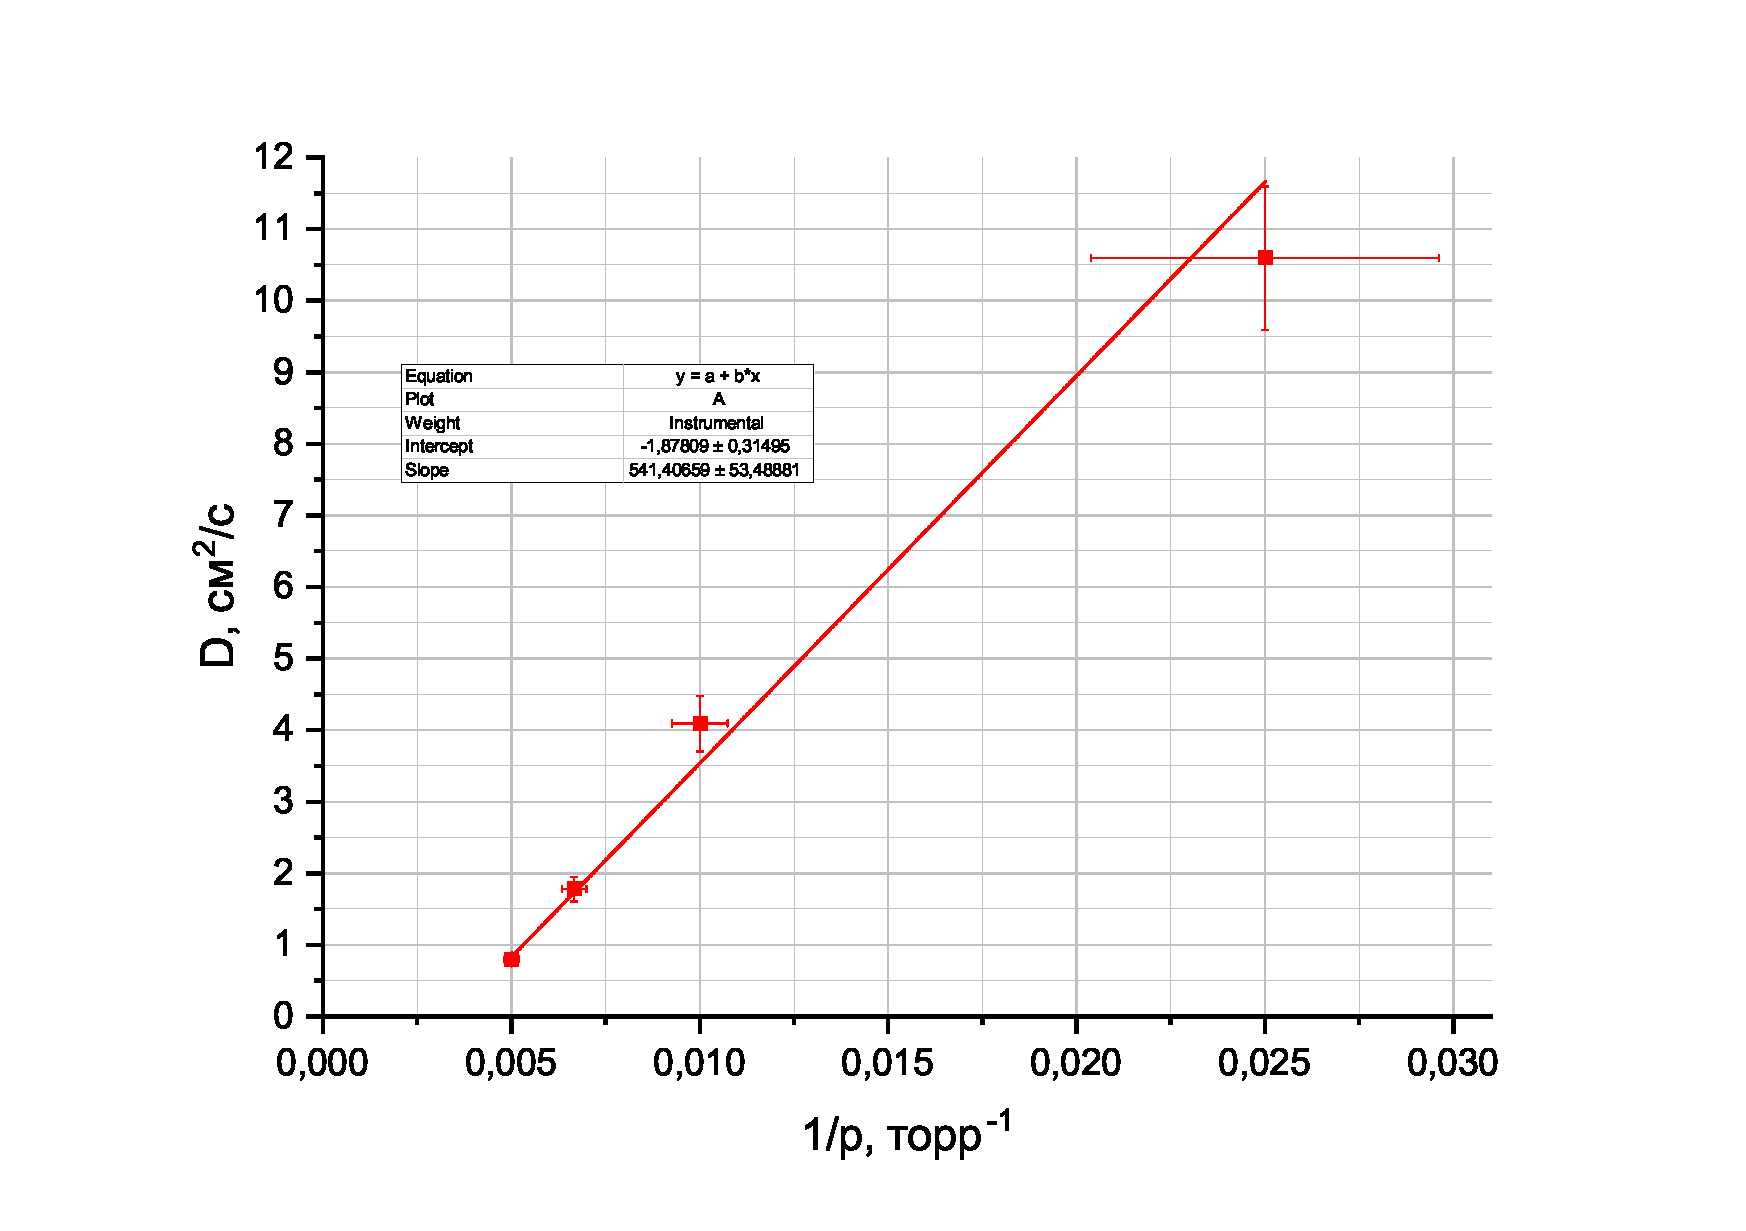
\includegraphics[width=\linewidth]{7}
    \caption{Определение главных направлений в пластинках}
    \label{fig:7}
\end{wrapfigure}

Поставим кристаллическую пластинку между скрещенными поляроидами
\ffig{fig:7}. Вращая пластинку вокруг направления луча и наблюдая за
интенсивностью света, проходящего сквозь второй поляроид, определим,
при каком условии главные направления пластинки совпадают с
разрешенными направлениями поляроидов. 

Собственные направления выделены тем, что световые волны, линейно
поляризованные в этих направлениях, распространяются в кристалле,
сохраняя свое состояние поляризации. То есть вращением пластинки мы
ищем два положения, где в скрещенных поляроидах происходит полное
затемнение. Это означает, что линейно поляризованная волна (после
прохождения поляроида $P_1$) никак не изменяет своей поляризации,
соответственно такая волна не пройдет через поляроид $P_2$, а
направлении главной оси совпадает с ориентацией поляроида $P_1$.

Повторим опыт для второй
пластинки.

\subsection*{Пластинки $\lambda/2,\ \lambda/4$}
Добавим к схеме, изображенной на \fig{fig:7}, зеленый фильтр.
Установим разрешенное направление первого поляроида горизонтально, а
главные направления исследуемой пластинки --- под углом $45^\circ$ к
горизонтали. 

С помощью второго поляроида установим, какую поляризацию имеет свет,
прошедший пластинку: круговую или линейную с переходом в другой
квадрант. 

Если при всех положениях второго поляроида $P_2$ мы не наблюдаем полного
затемнения, то в оптической схеме находится пластинка $\lambda/4$, так
как она создает круговую поляризацию. Если же при определённом
положении второго поляроида $P_2$, свет не проходит через поляроид, то
перед нами пластинка $\lambda/2$, которая просто поворачивает линейную
поляризацию на $90^\circ$.

\subsection*{Определение направлений большей и меньшей скорости в
пластинке}
Поставим между скрещенными поляроидами пластинку чувствительного
оттенка ($\lambda$ для зеленого света), имеющую вид стрелки. Световой
вектор, ориентированный вдоль направления стрелки, проходит с большей
скоростью, перпендикулярный с меньшей.

Установим разрешенное направление первого поляроида горизонтально и
убедимся с помощью второго поляроида, что эта пластинка не меняет
поляризацию зеленого света в условиях предыдущего опыта. Это связано с
тем, что пластинка толщиной $\lambda$ создает разность фаз между
волнами $\Delta \phi = 2\pi$, то есть поляризация не изменяется.

\begin{wrapfigure}{r}{0.4\linewidth}
    \vspace{-10pt}
    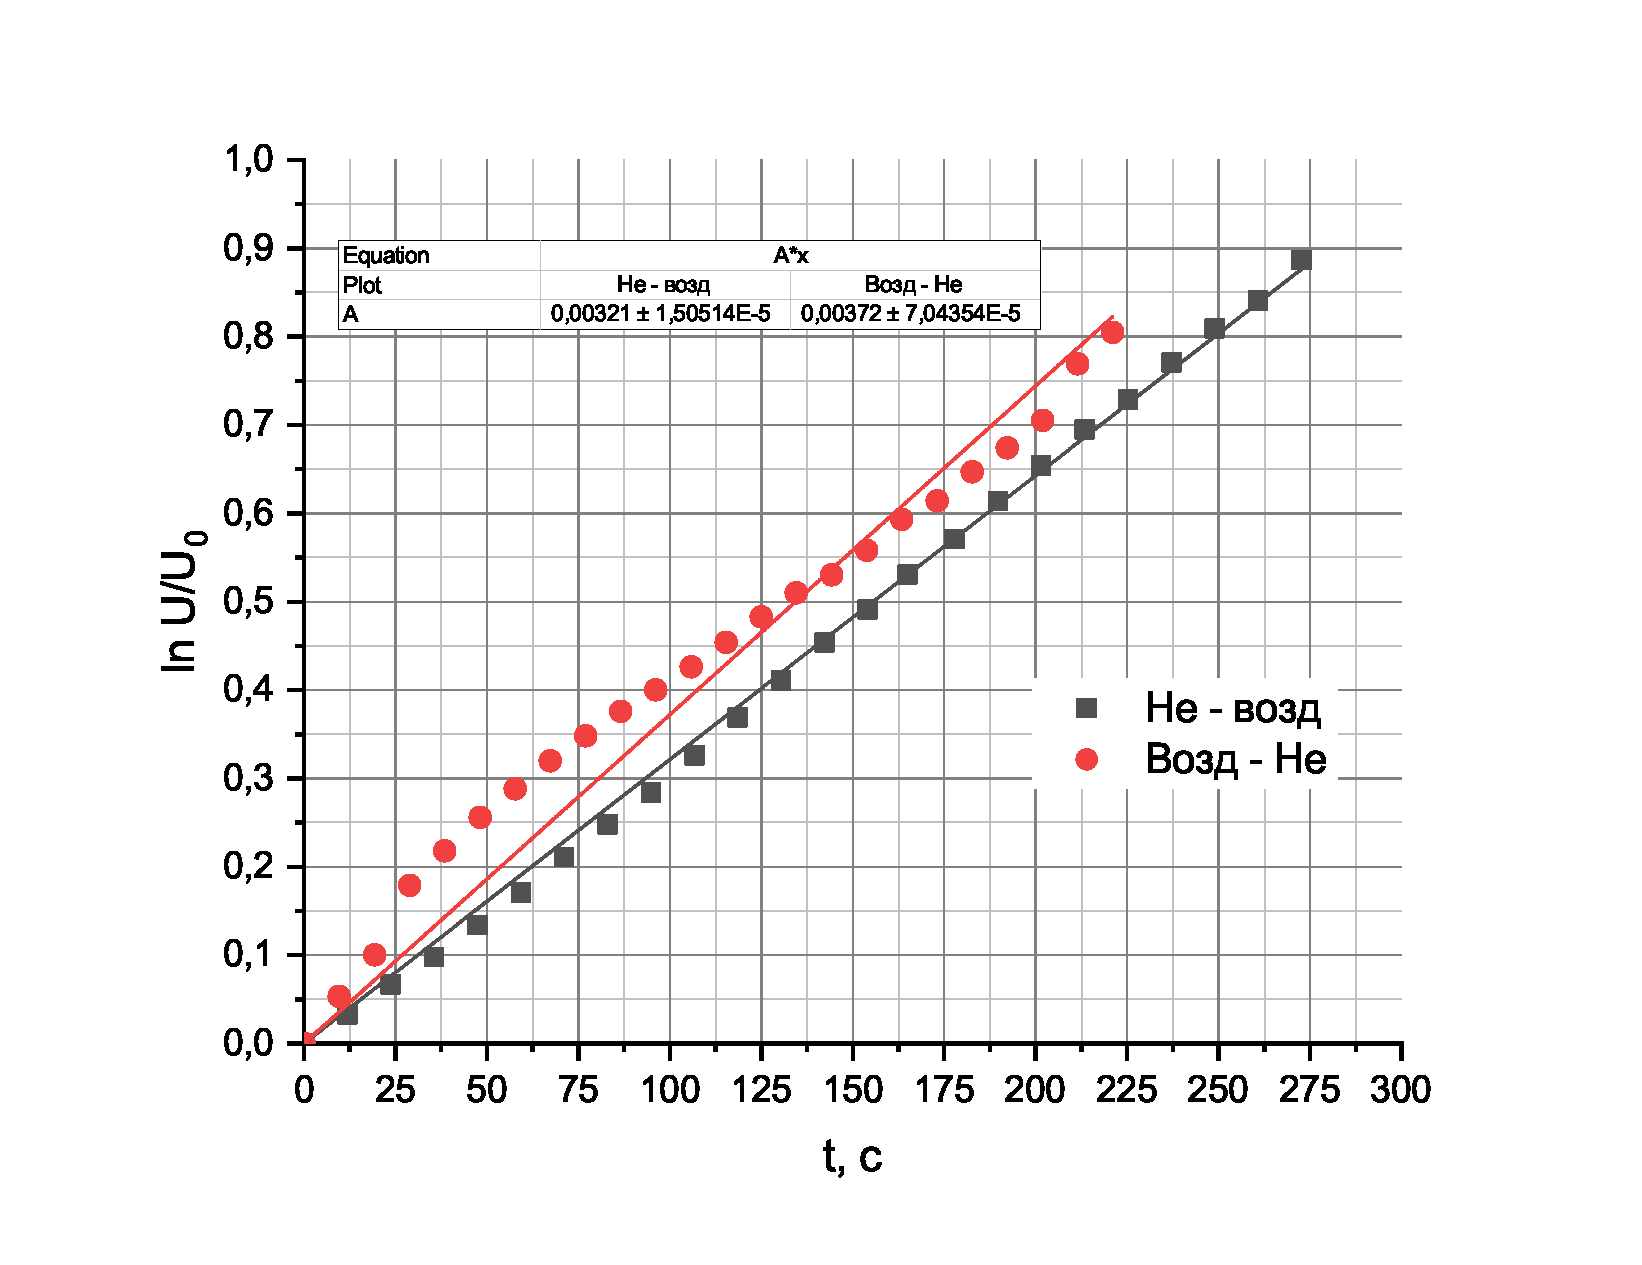
\includegraphics[width=\linewidth]{8}
    \caption{Определение направлений большей и меньшей скорости}
    \label{fig:9}
\end{wrapfigure}

Уберем зеленый фильтр и поставим между скрещенными поляроидами
пластинку $\lambda$ (стрелка под углом $45^\circ$ к разрешенным
направлениям поляроидов). Глядя сквозь второй поляроид на стрелку,
убеждаемся, что она имеет пурпурный цвет (зеленый свет задерживается
вторым поляроидом, а красная и синяя компоненты проходят). 

Добавим к схеме пластинку $\lambda/4$ \ffig{fig:9}, главные
направления которой совпадают с главными направлениями пластины
$\lambda$ и ориентированы под углом $45^\circ$ к разрешенным
направлениям скрещенных поляроидов.

При повороте рейтера со стрелкой на $180^\circ$ вокруг вертикальной
оси цвет стрелки меняется от зелено-голубого до оранжево-желтого.

Это соответствует разности хода в $\lambda$ для света с
большей длиной волны. При освещении этих пластинок белым светом теперь
погасится не зеленая, а красная часть спектра, и проходящий свет будет
казаться зеленовато-голубым. Если же главные направления,
соответствующие большей скорости распространения, у пластинки
чувствительного оттенка и у пластинки в $\lambda/4$ окажутся
перпендикулярными, то проходящий свет приобретет оранжево-желтую
окраску. Следовательно, в первом случае у нас <<быстрая>> ось (они
совпадают), во втором ---медленная.

\section*{Интерференция поляризованных лучей}
Расположим между скрещенными поляроидами мозаичную слюдяную пластинку.
Она собрана из 4-х узких полосок слюды, лежащих по сторонам квадрата
(две полоски толщиной $\lambda/4$ и по одной --- $\lambda/2$ и
$3\lambda/4$). В центральном квадрате слюды нет. Главные направления
всех пластинок ориентированы параллельно сторонам квадрата.

Итого получаются квадратики с толщиной: $0, \frac{\lambda}{4},
\frac{\lambda}{2}, \frac{3\lambda}{4}, \lambda$. 
\renewcommand{\labelenumi}{\theenumi)}
\renewcommand{\theenumi}{\asbuk{enumi}}
\begin{enumerate}
    \item При вращении
пластинки цвет квадратиков не изменяется, так как амплитуды и
разности фаз не изменяются. Меняется только
интенсивность квадратиков.

Когда главное направление пластин совпадает с направлением
поляризации задаваемым поляроидом $P_1$, все квадратики
становятся темными (за один оборот это случается 4 раза), то есть
интенсивность минимальна, так как
при этом ни одна пластинка не меняет поляризацию света.

%Окрашены только угловые квадратики
%\begin{itemize}
%    \item Центральный квадратик (без слюды) при любом положении
%пластинки будет темным, так как поляроиды скрещены и свет без
%изменения поляризации не проходит.
%\item Два квадратика окрашены в оранжевый цвет 
%\end{itemize}
%    \item 
\item При повороте на $45^\circ$ цвета исчезают. Это связано с тем что
    угол поворота главных направлений пластинок совпадает с углом
    поворота поляроида $P_2$.

    Поворачивая поляроид $P_2$ на $90^\circ$ окраска пластинки
    меняется на дополнительную (красный на голубой, зеленый на
    фиолетовый, синий на желтый и т.д.)
\end{enumerate}



\begin{figure}[H]
    \floatsetup{heightadjust=object,valign=c}
    \begin{floatrow}

        \ffigbox{
        \caption{Поляроиды скрещены, пластинка находится под углом
        $45^\circ$}
    }
        {
        \includegraphics[width=0.6\linewidth]{9}
    }

        \ffigbox{
            \caption{Второй поляроид $P_2$ как и пластинка наклонены
            под углом $45^\circ$ относительно первого поляроида $P_1$}
    }
        {
        \includegraphics[width=0.6\linewidth]{10}
    }
    \end{floatrow}
\end{figure}




%\subsection*{Определение направления вращения светового вектора в
%эллиптически поляризованной волне}
%Нарисуем эллипс поляризации для вектора $\vv{E}$, вышедшего из
%пластинки $\lambda/4$. Ось $x$ соответствует большей скорости. Рядом
%нарисуем две вышедших из пластинки синусоиды $x(t)$ и $y(t)$ со
%сдвигом фаз в четверть периода. Определим нападение вращения
%электрического вектора в эллиптически поляризованной волне.
%
%\begin{figure}[H]
%    \begin{tikzpicture}[>=Stealth]
%%\datavisualization [>=Stealth]
%%\datavisualization[format=function]
%\draw (2,0) ellipse [x radius=2, y radius=1];
%\draw[->]
%    (2,-1.5) -- (2,1.5);
%\draw[->]
%    (-1,0) --  (5,0);
%\node (a) at (5,0.2) {$x$};
%\node (b) at (2.3,1.5) {$y$};
%
%\draw[->] (7,0) -- (13,0) node[right] {$x$};
%\draw[->] (10,-1.2) -- (10,1.2) node[above] {$f(x)$};
%%\draw[color=red] plot[id=x-10] function{x-10};
%\end{tikzpicture}
%\caption{Эллипс поляризации и графики синусоид}
%\label{fig:9}
%\end{figure}
%
%\begin{tikzpicture}[domain=0:4]
%\draw[very thin,color=gray] (-0.1,-1.1) grid (3.9,3.9);
%\draw[->] (-0.2,0) -- (4.2,0) node[right] {$x$}; \draw[->] (0,-1.2) -- (0,4.2) node[above] {$f(x)$};
%\draw[color=red] plot[id=x] function{x} node[right] {$f(x) =x$};
%\draw[color=blue] plot[id=sin] function{sin(x)} node[right] {$f(x) = \sin x$}; \draw[color=orange] plot[id=exp] function{0.05*exp(x)} node[right] {$f(x) = \frac{1}{20} \mathrm e^x$};
%\end{tikzpicture}


\section{Обсуждение результатов и выводы}
В работе был измерен угол Брюстера для эбонита:
\[
    \theta = (53\pm 2)^\circ
\]
По значению угла Брюстера был рассчитан показатель преломления эбонита.
\[
    n=1,33\pm 0,10
\]
Табличное значение:
\[
    n_{\text{т}} = 1,6-1,7
\]

Измеренное значение отличается от табличного. Несовпадение связано с
тем, что наблюдения проводились с помощью глаза, положение которого мы
не можем зафиксировать, соответственно не соблюдаем схему опыта на \fig{fig:5}

В работе был исследован метод разделения монохроматического света на
$s$ и $p$-поляризованный. Стопа стеклянных пластинок (\fig{fig:6})
выделяет $s$-компоненту, что видно по второму поляроиду $P_2$, и
пропускает $p$-компоненту, что видно по первому поляроиду $P_1$. Угол
между поляроидами равен $\pi/2$.

Были рассмотрены двоякопреломляющие пластинки, позволяющие изменять
поляризацию света. С помощью скрещенных поляроидов можно определить
тип поляризации после прохождения пластинки, а также главные
направления пластин. Пластинка $\lambda/4$
преобразует линейную
поляризацию в круговую, а $\lambda/2$ поворачивает линейную
поляризацию на $\pi/2$.

При исследовании естественного света с помощью пластинки
чувствительного оттенка были определены быстрая и медленная оси
пластинки.

При использовании пластинок разной длины волны в скрещенных
поляроидах можно наблюдать явление интерференции, которое проявляется
в окраске изначально прозрачных пластин.


\end{document}
